\chapter{Further discussions}
The previous chapter presented results that indicated A* search using priority queue from the C++ standard template library has the best performance.
The results also shows that shortest path calculations can be speed up further when it is in an iterative environment.
In this chapter we discuss the details behind the mentioned results,
including why some of the algorithms that should have performed better but failed to do so.

\section{Priority queues}
The priority queue implementation results showed that
all of the heap implementations from the Boost library is worse than $\langle$priority\_queue$\rangle$.
The reason behind this can be explained using the Binary heap implementation.
It turns out that the implementation of $\langle$priority\_queue$\rangle$ is almost similar to Binary heap from the Boost library,
the only difference is their underlying storage of node information.
Nodes are stored using an array in the standard library version,
where as the Boost library uses pointers to keep track of 
the nodes.
Due to computer cache coherence,
it is known that accessing data from a nearby memory (RAM) locations in a short period of time is faster than accessing from distant memory locations.
This is due to cache memory access being much faster than RAM access,
and internally a block of memory are pre-fetched into the cache in a hope they will be accessed in a short period of time).
In the shortest path algorithms,
the Heap tree need to be searched over and over in a short period of time when nodes are being scanned and inserted.
The standard library version uses an array where data are stored linearly in a nearby location,
so it is much faster than the pointer based version where memory are allocated in random locations when nodes are inserted.

\subsection{Fibonacci heap}
Here we discuss the reason behind Fibonacci heap not performing well despite its $O(1)$ amortized time Decrease-Key operation.
As described in the two priority queue sections (Section~\ref{sec:pq} and \ref{sec:pq_implementation}),
the Decrease-Key operation is used to change the distance label of a node when the node is already in the heap.
It was discovered that the $O(1)$ time has a very high constant factor,
and Fibonacci heap only works well if the underlying graph is large and dense (i.e.\ every node connects to almost every other node).
This discovery comes from the fact that 
the Decrease-Key operation is only used frequent when the graph is dense,
so cumulatively its high constant $O(1)$ time will perform better compared to $O(\log(N))$ time in other heap implementations, where $N$ need to be a large number.

Now we confirm our graph is indeed not dense and the Decrease-Key is not used frequent.
We find that all of our graphs are very sparse.
The degree of any node of any graph is no more than 5,
as it is already really rare to have an intersection with 5 roads connected.
The graphs only have about 0.4\% to 0.6\% of arcs in the corresponding complete graph (every node connects to every other node).
We also find that in all of the experimented graphs when using Dijkstra's algorithm,
the probability of using Decrease-Key on any node is around 1 to 5 percent.

\section{Bidirectional algorithms}
In this section we investigate the reason for the worse performances of the bidirectional algorithms. 

First we examine whether search areas of the algorithms are what is expected.
Figure~\ref{fig:long_sptree} shows the shortest path trees of the point-to-point algorithms, where the origin and destination node is placed on the opposite side of the ChicagoSketch network.
It can be seen that Dijkstra's algorithm scans the entire network.
Bidirectional Dijkstra scans almost the entire network with some nodes on the side left out.
Bidirectional A* scans a slightly larger region near the origin and destination nodes,
and the A* search scans just a few nodes along the shortest path.
The behaviour of the algorithms is shown further in Figure~\ref{fig:short_sptree},
where the origin and destination is placed close to each other.
It is shown that both Dijkstra's algorithm and its bidirectional version scan almost half of the graph,
where bidirectional search scans less.
A* and its bidirectional search scan a small portion of the graph,
and they do not scan the area behind the origin and destination node compared to the Dijkstra's algorithm.

The search areas of the Dijkstra's algorithms match what is expected,
but not the run times.
The reason for reduction in run time is due to our implementations.
In both forward and backward search,
the current shortest path $\mu$ need to be updated every time a node is scanned,
and the stopping criterion need to be checked when a node is labelled.
Furthermore,
once the algorithm terminates,
we need to retrieve the shortest path in both directions by following their predecessors and concatenate them together for the full shortest.
So it is concluded that these addition computations slowed down the run times.

For A* search,
the bidirectional version scans more nodes than the unidirectional version.
And since the bidirectional version has similar stopping criterion compared to the bidirectional Dijkstra's algorithm,
it is easy to understand why bidirectional A* performed worse.

\begin{figure}
    \centering
    \begin{subfigure}{.5\textwidth}
        \centering
        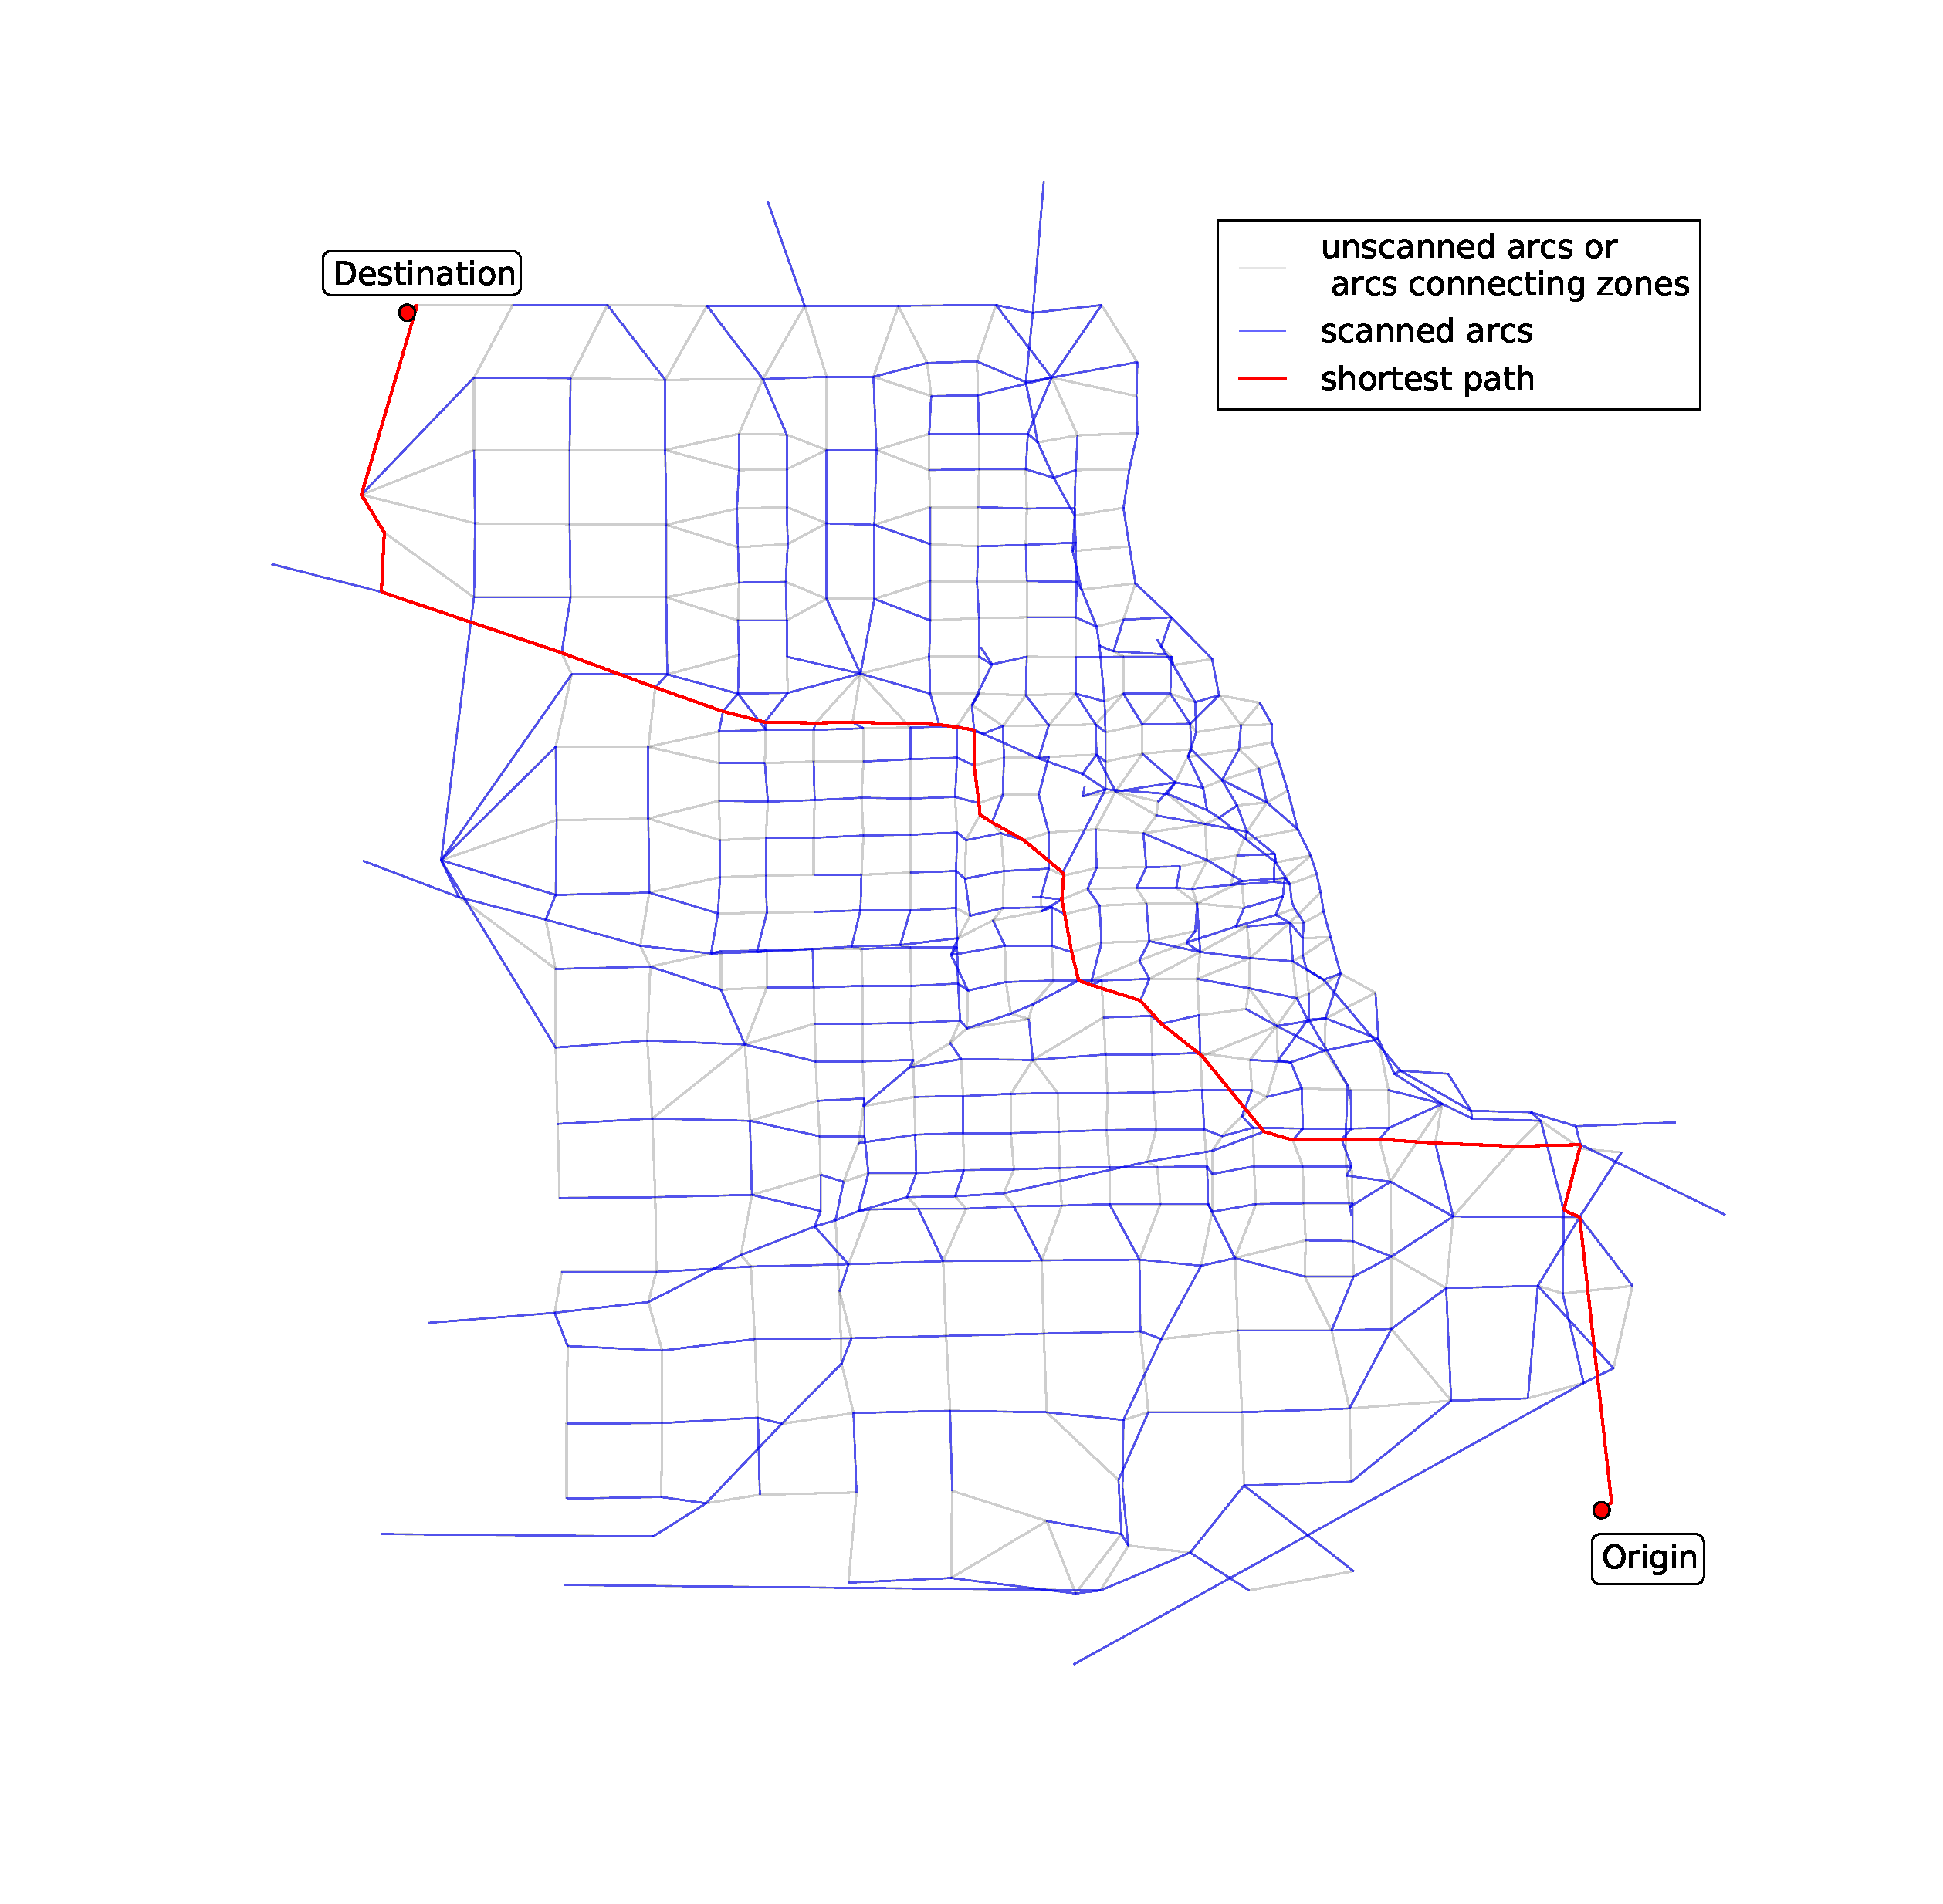
\includegraphics[width=\textwidth,trim=120px 120px 48px 120px,clip]{img/chicago_dijkstra}
        \caption{Dijkstra}
        \label{fig:chicago_dijkstra}
    \end{subfigure}%
    \begin{subfigure}{.5\textwidth}
        \centering
        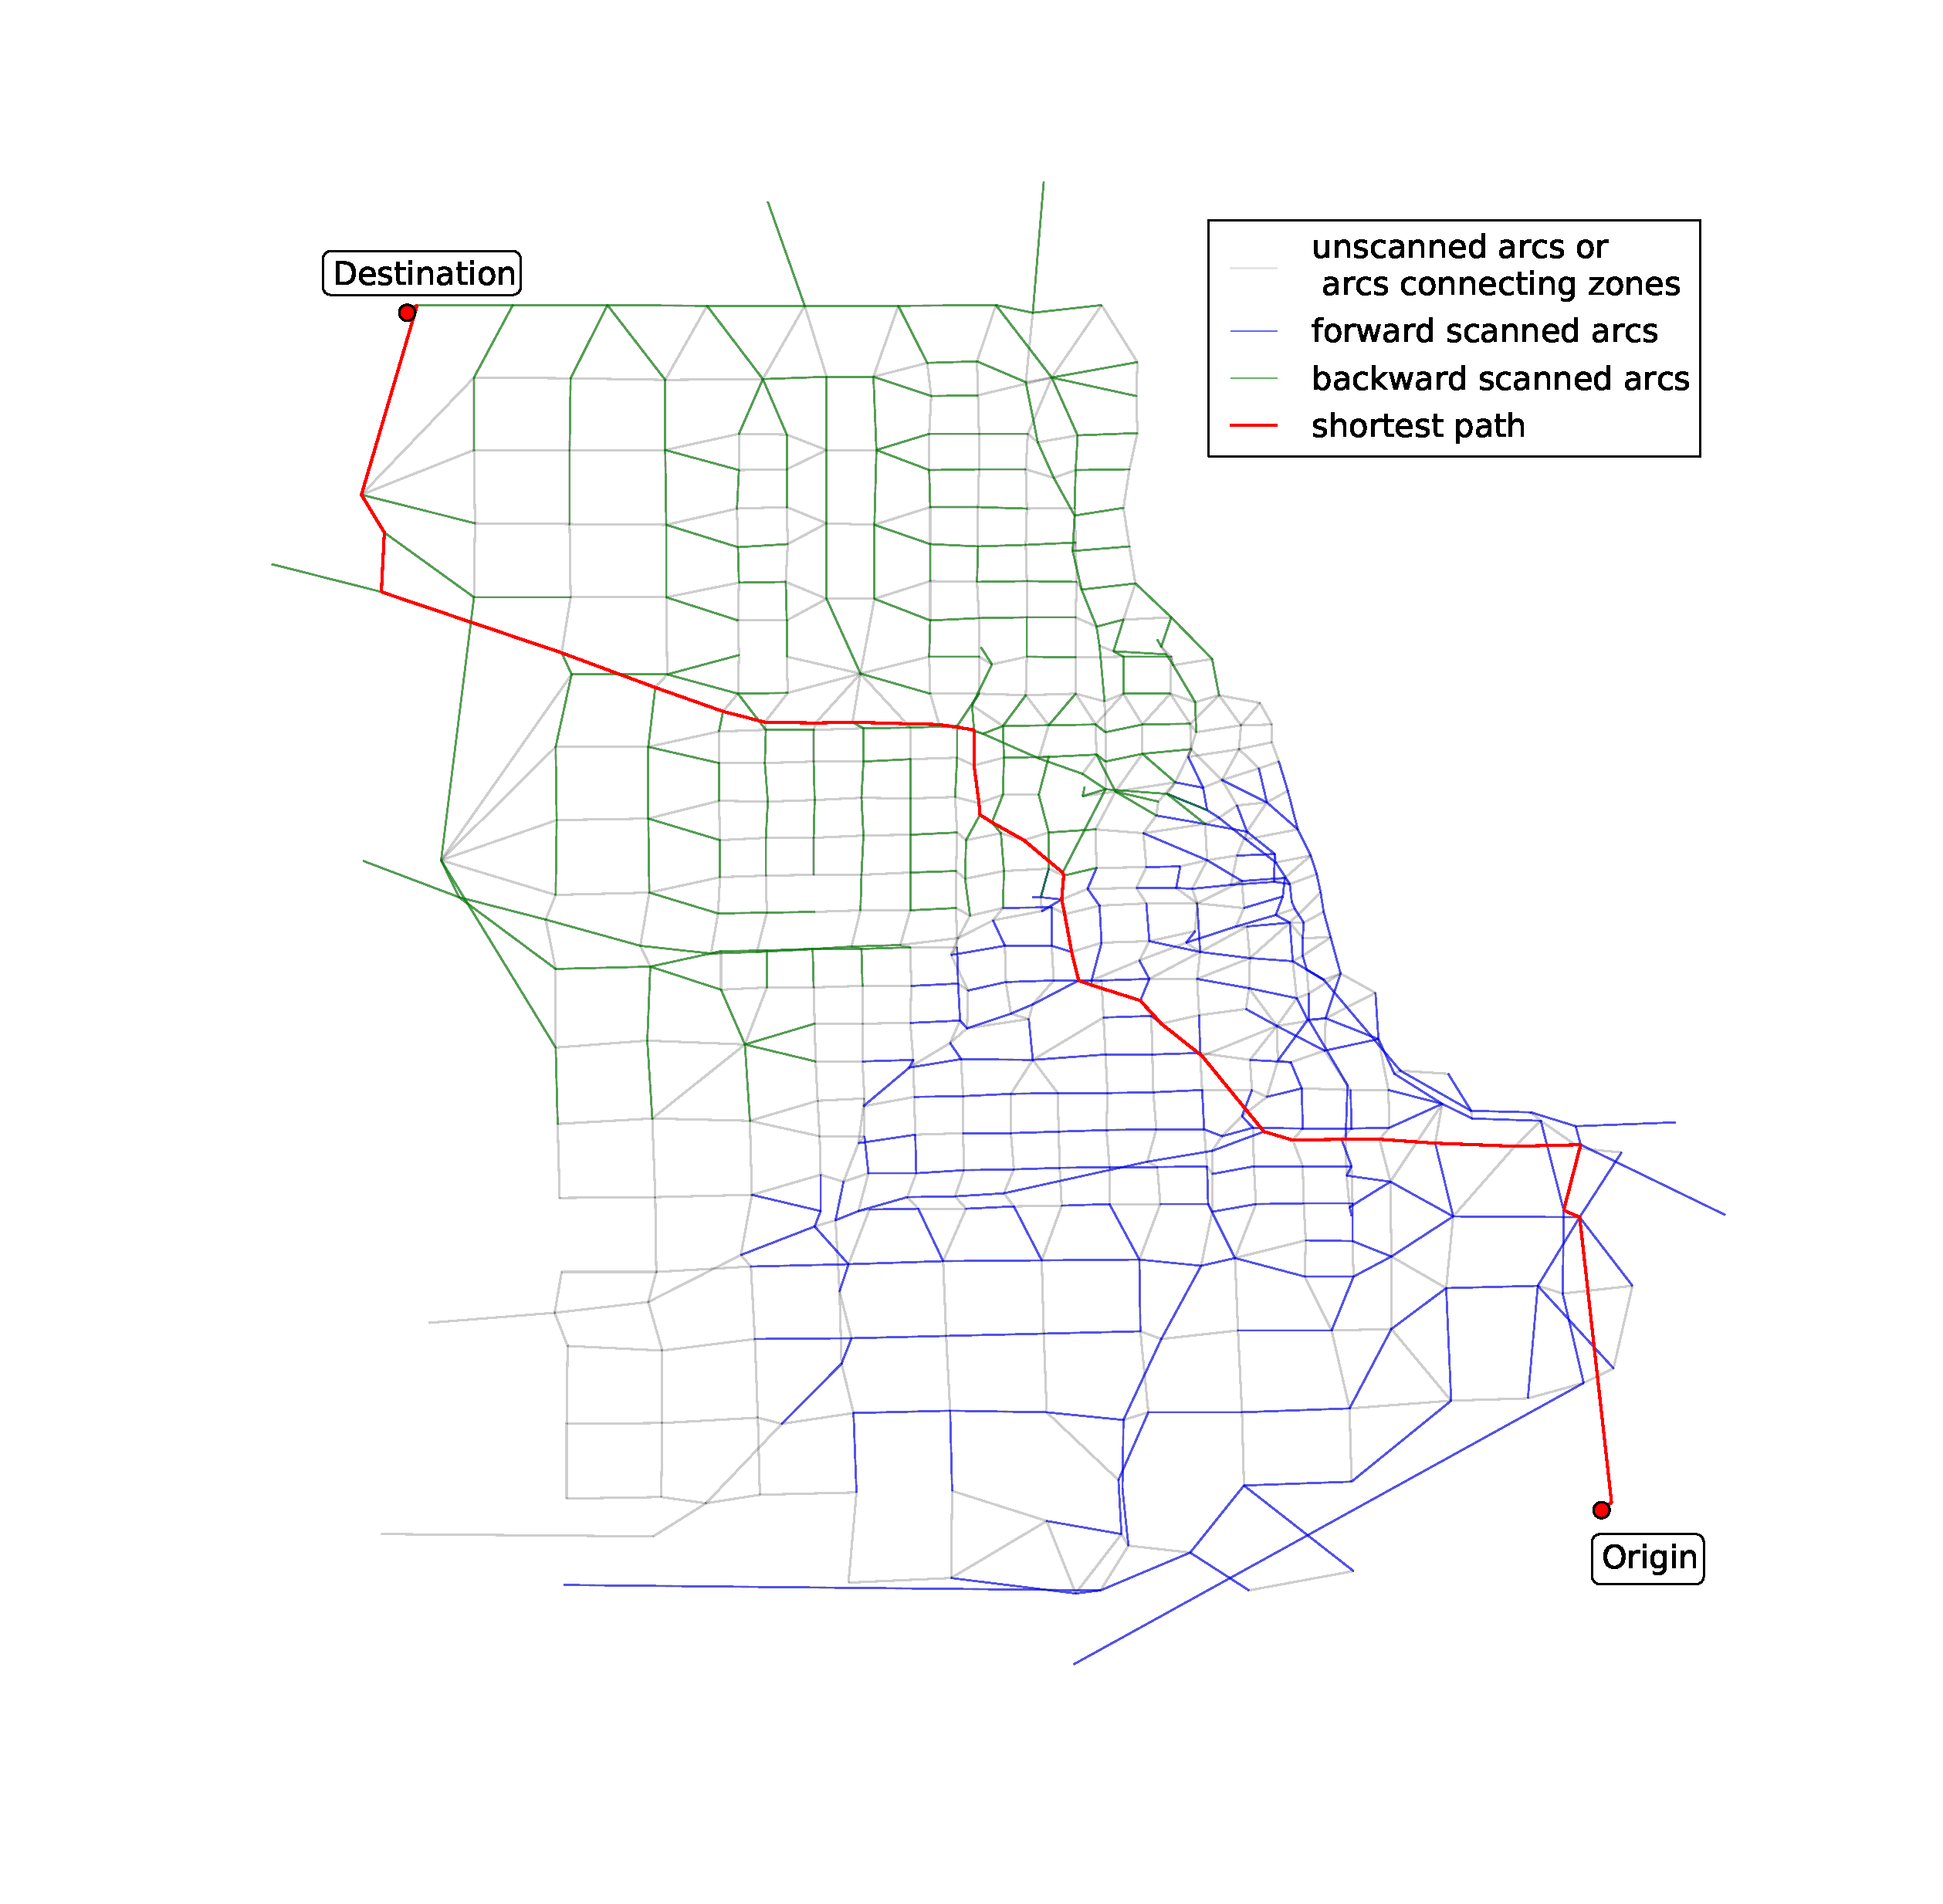
\includegraphics[width=\textwidth,trim=120px 120px 48px 120px,clip]{img/chicago_bidirect}
        \caption{Bidirectional Dijkstra}
        \label{fig:chicago_bidirect}
    \end{subfigure}
    \begin{subfigure}{.5\textwidth}
        \centering
        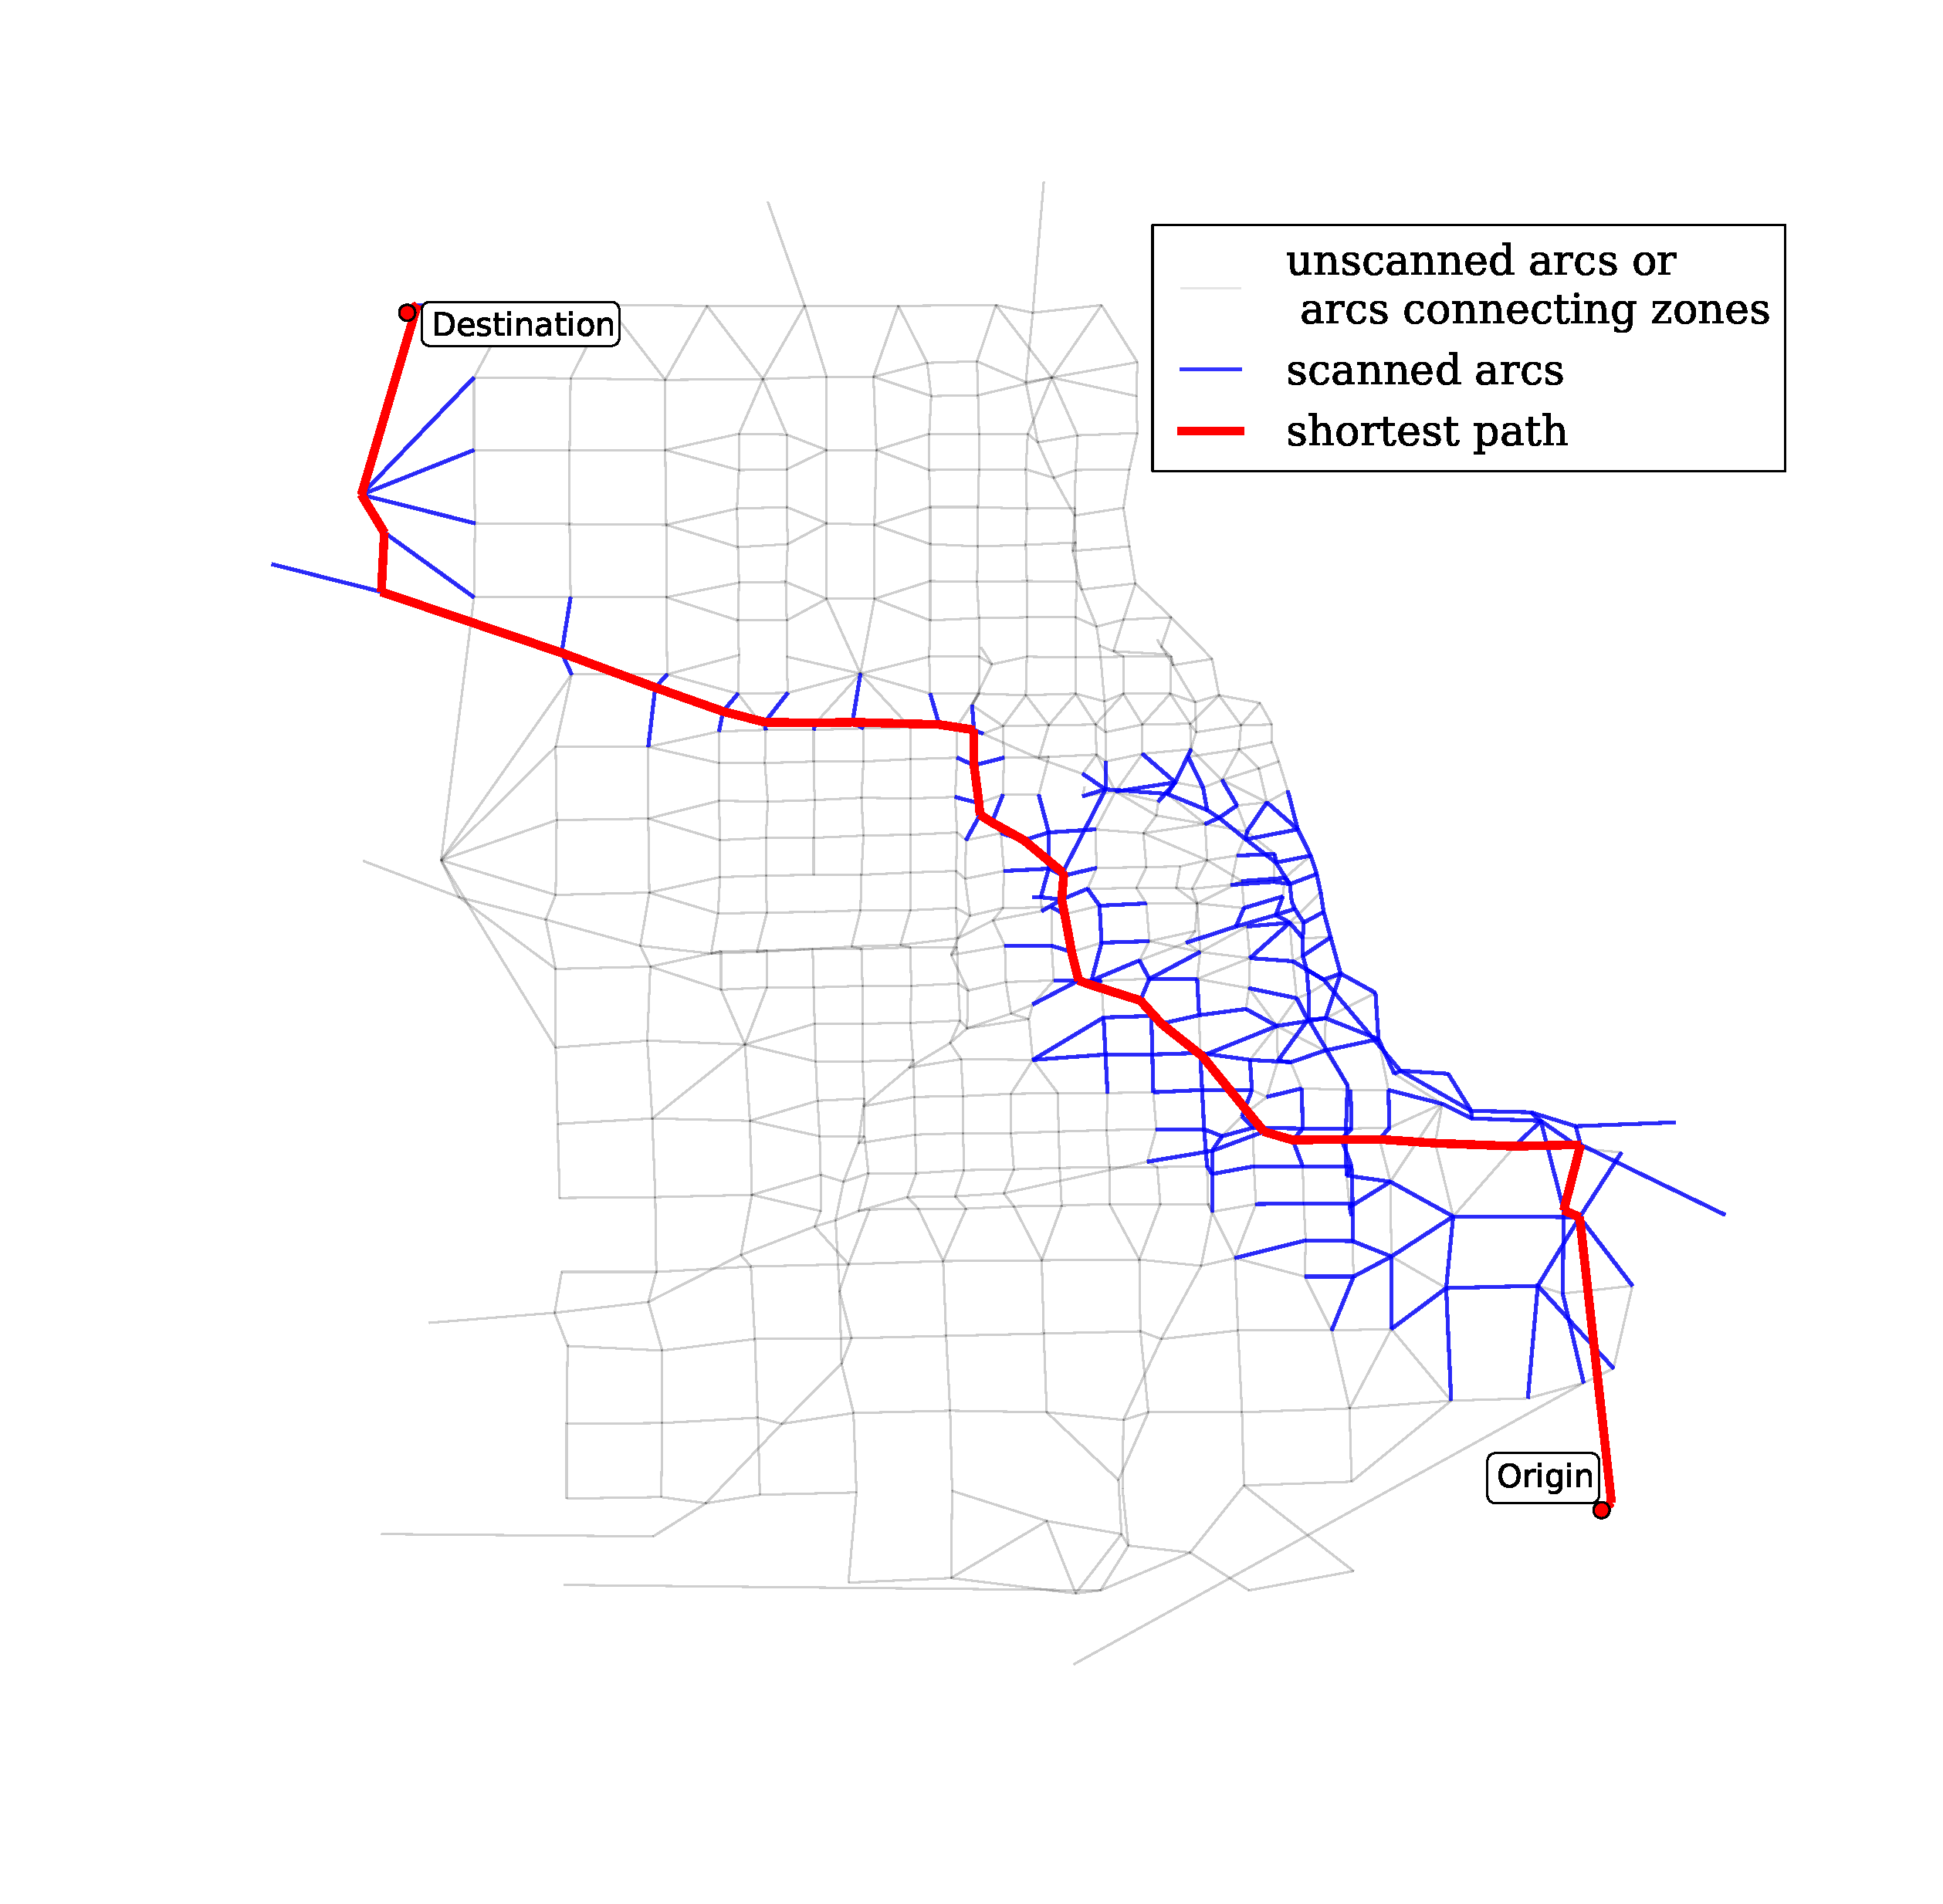
\includegraphics[width=\textwidth,trim=120px 120px 48px 0px,clip]{img/chicago_astar}
        \caption{A* Search}
        \label{fig:chicago_astar}
    \end{subfigure}%
    \begin{subfigure}{.5\textwidth}
        \centering
        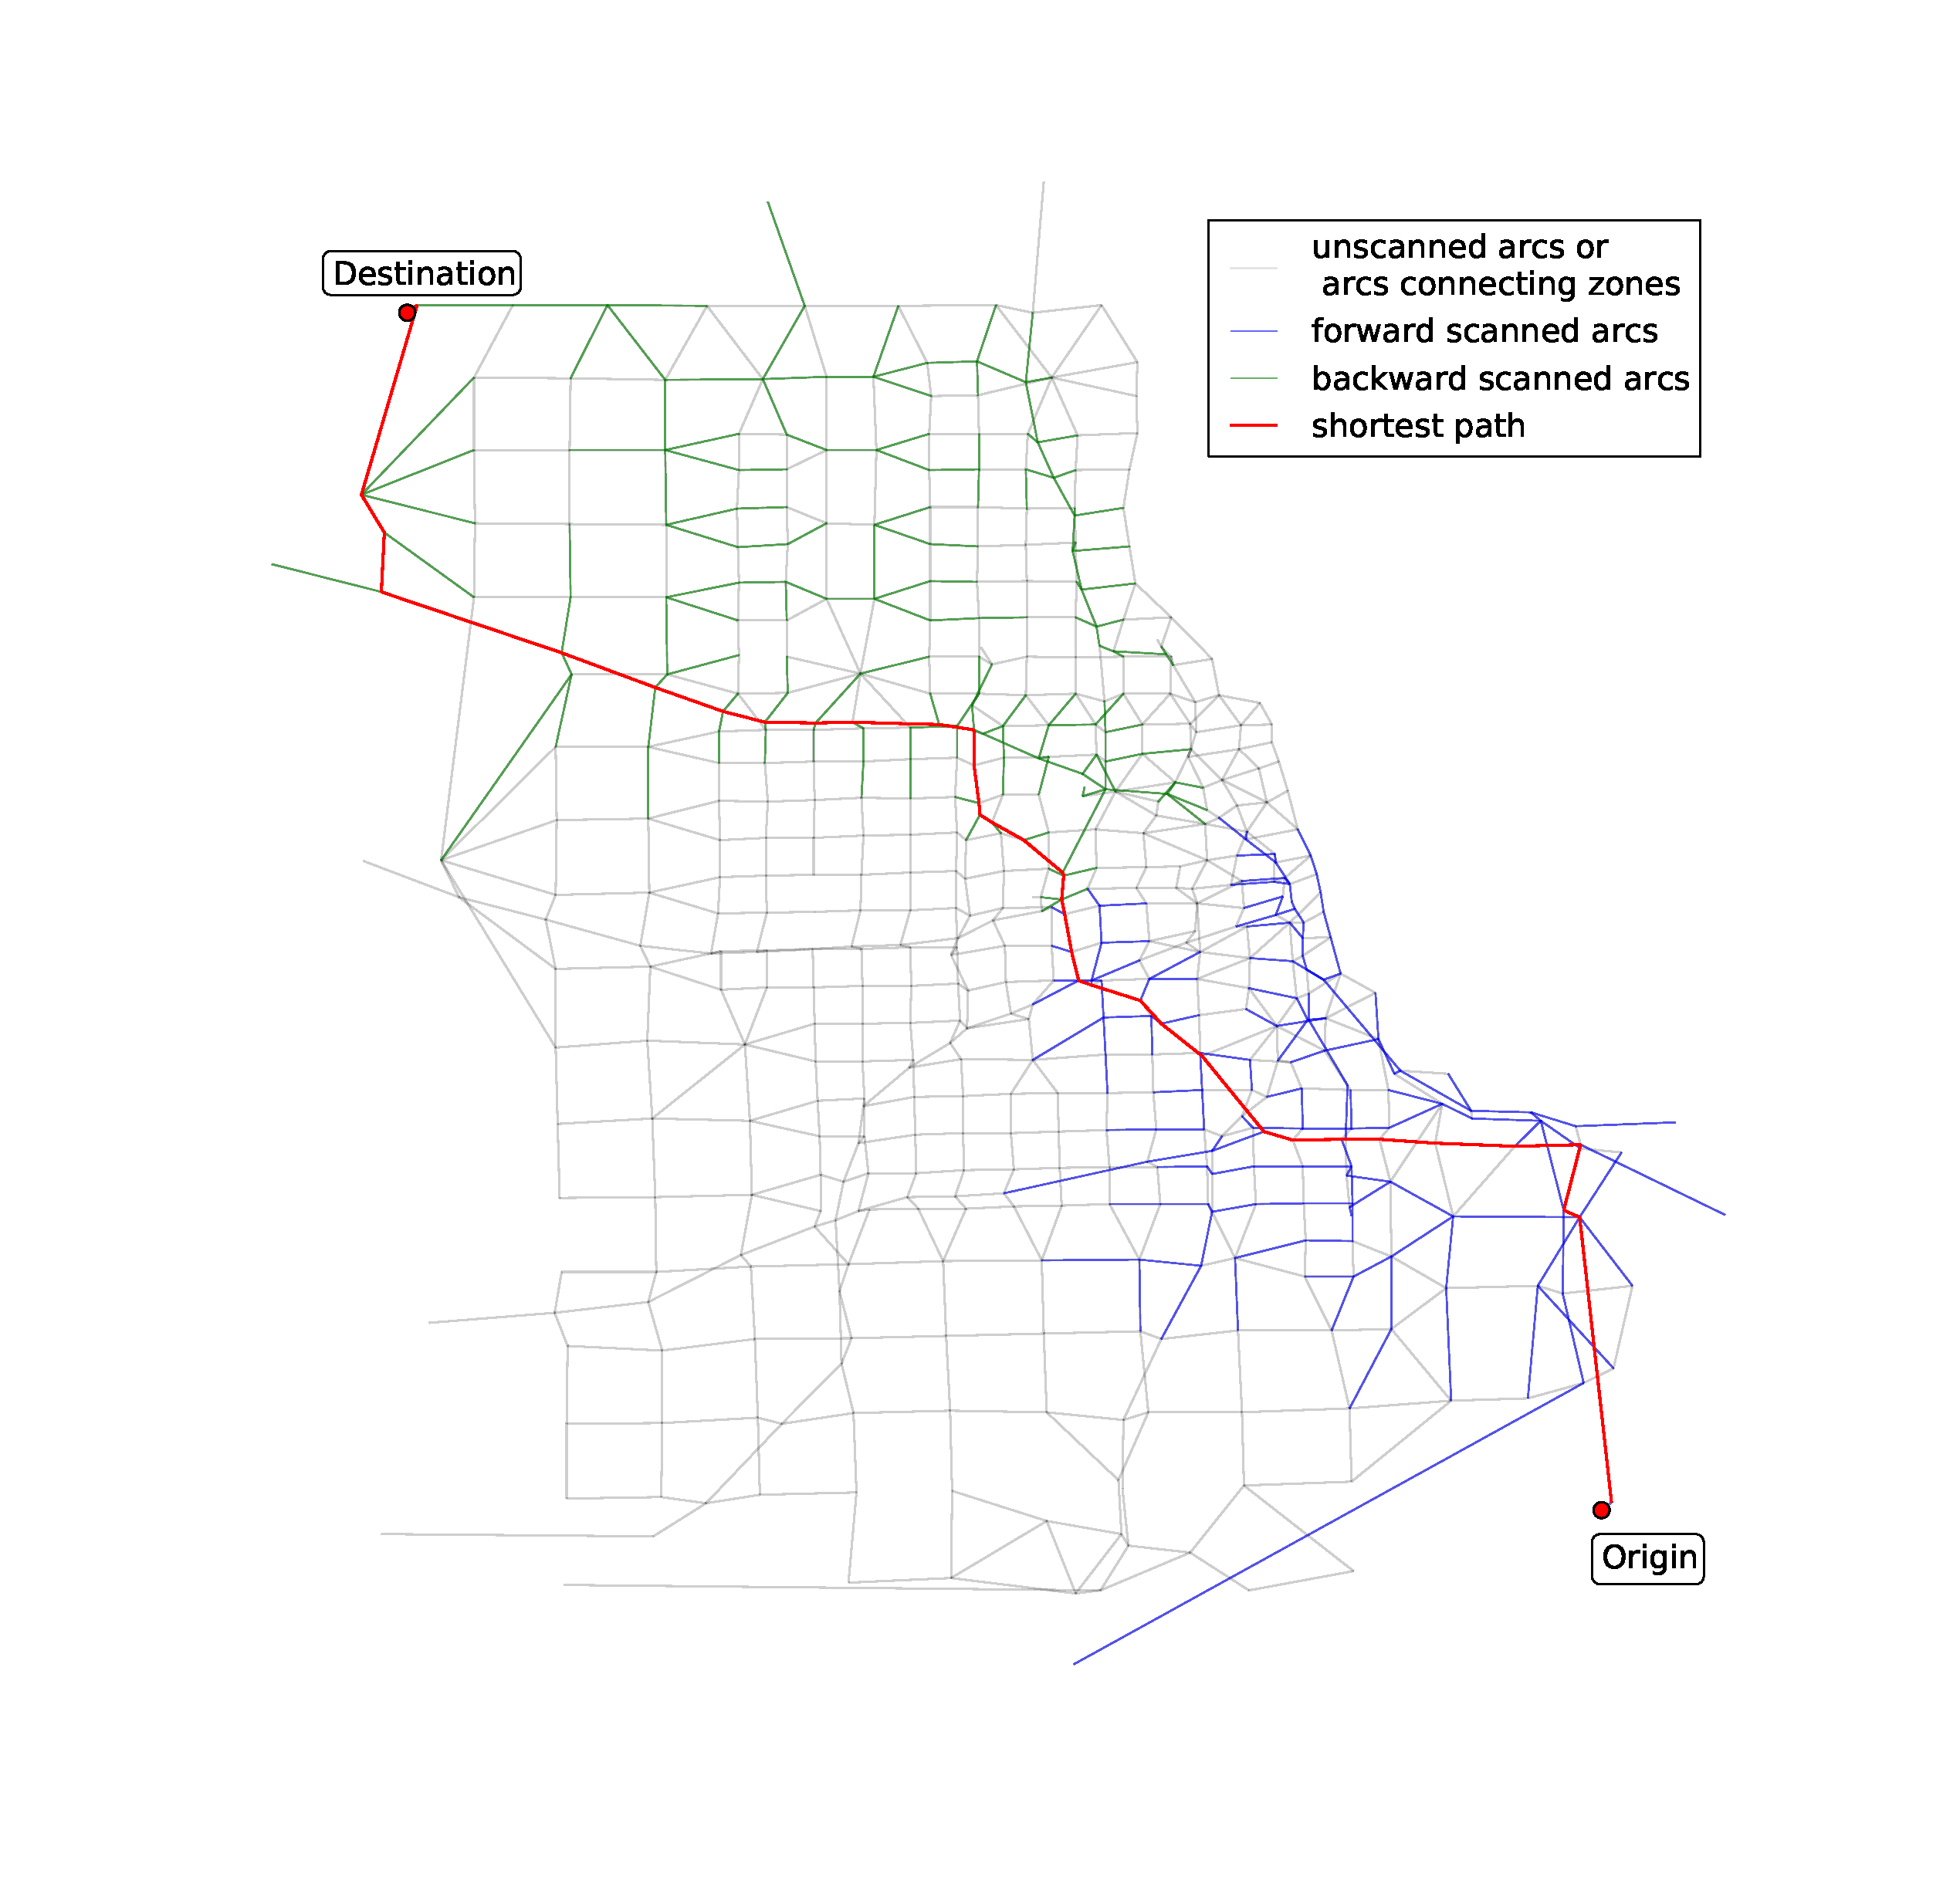
\includegraphics[width=\textwidth,trim=120px 120px 48px 0px,clip]{img/chicago_astar_bidirect}
        \caption{Bidirectional A* Search}
        \label{fig:chicago_astar_bidirect}
    \end{subfigure}
    \vspace{1em}
    \caption{Shortest path tree between two distant nodes in the ChicagoSketch Network}
    \label{fig:long_sptree}
\end{figure}

\begin{figure}
    \centering
    \begin{subfigure}{.5\textwidth}
        \centering
        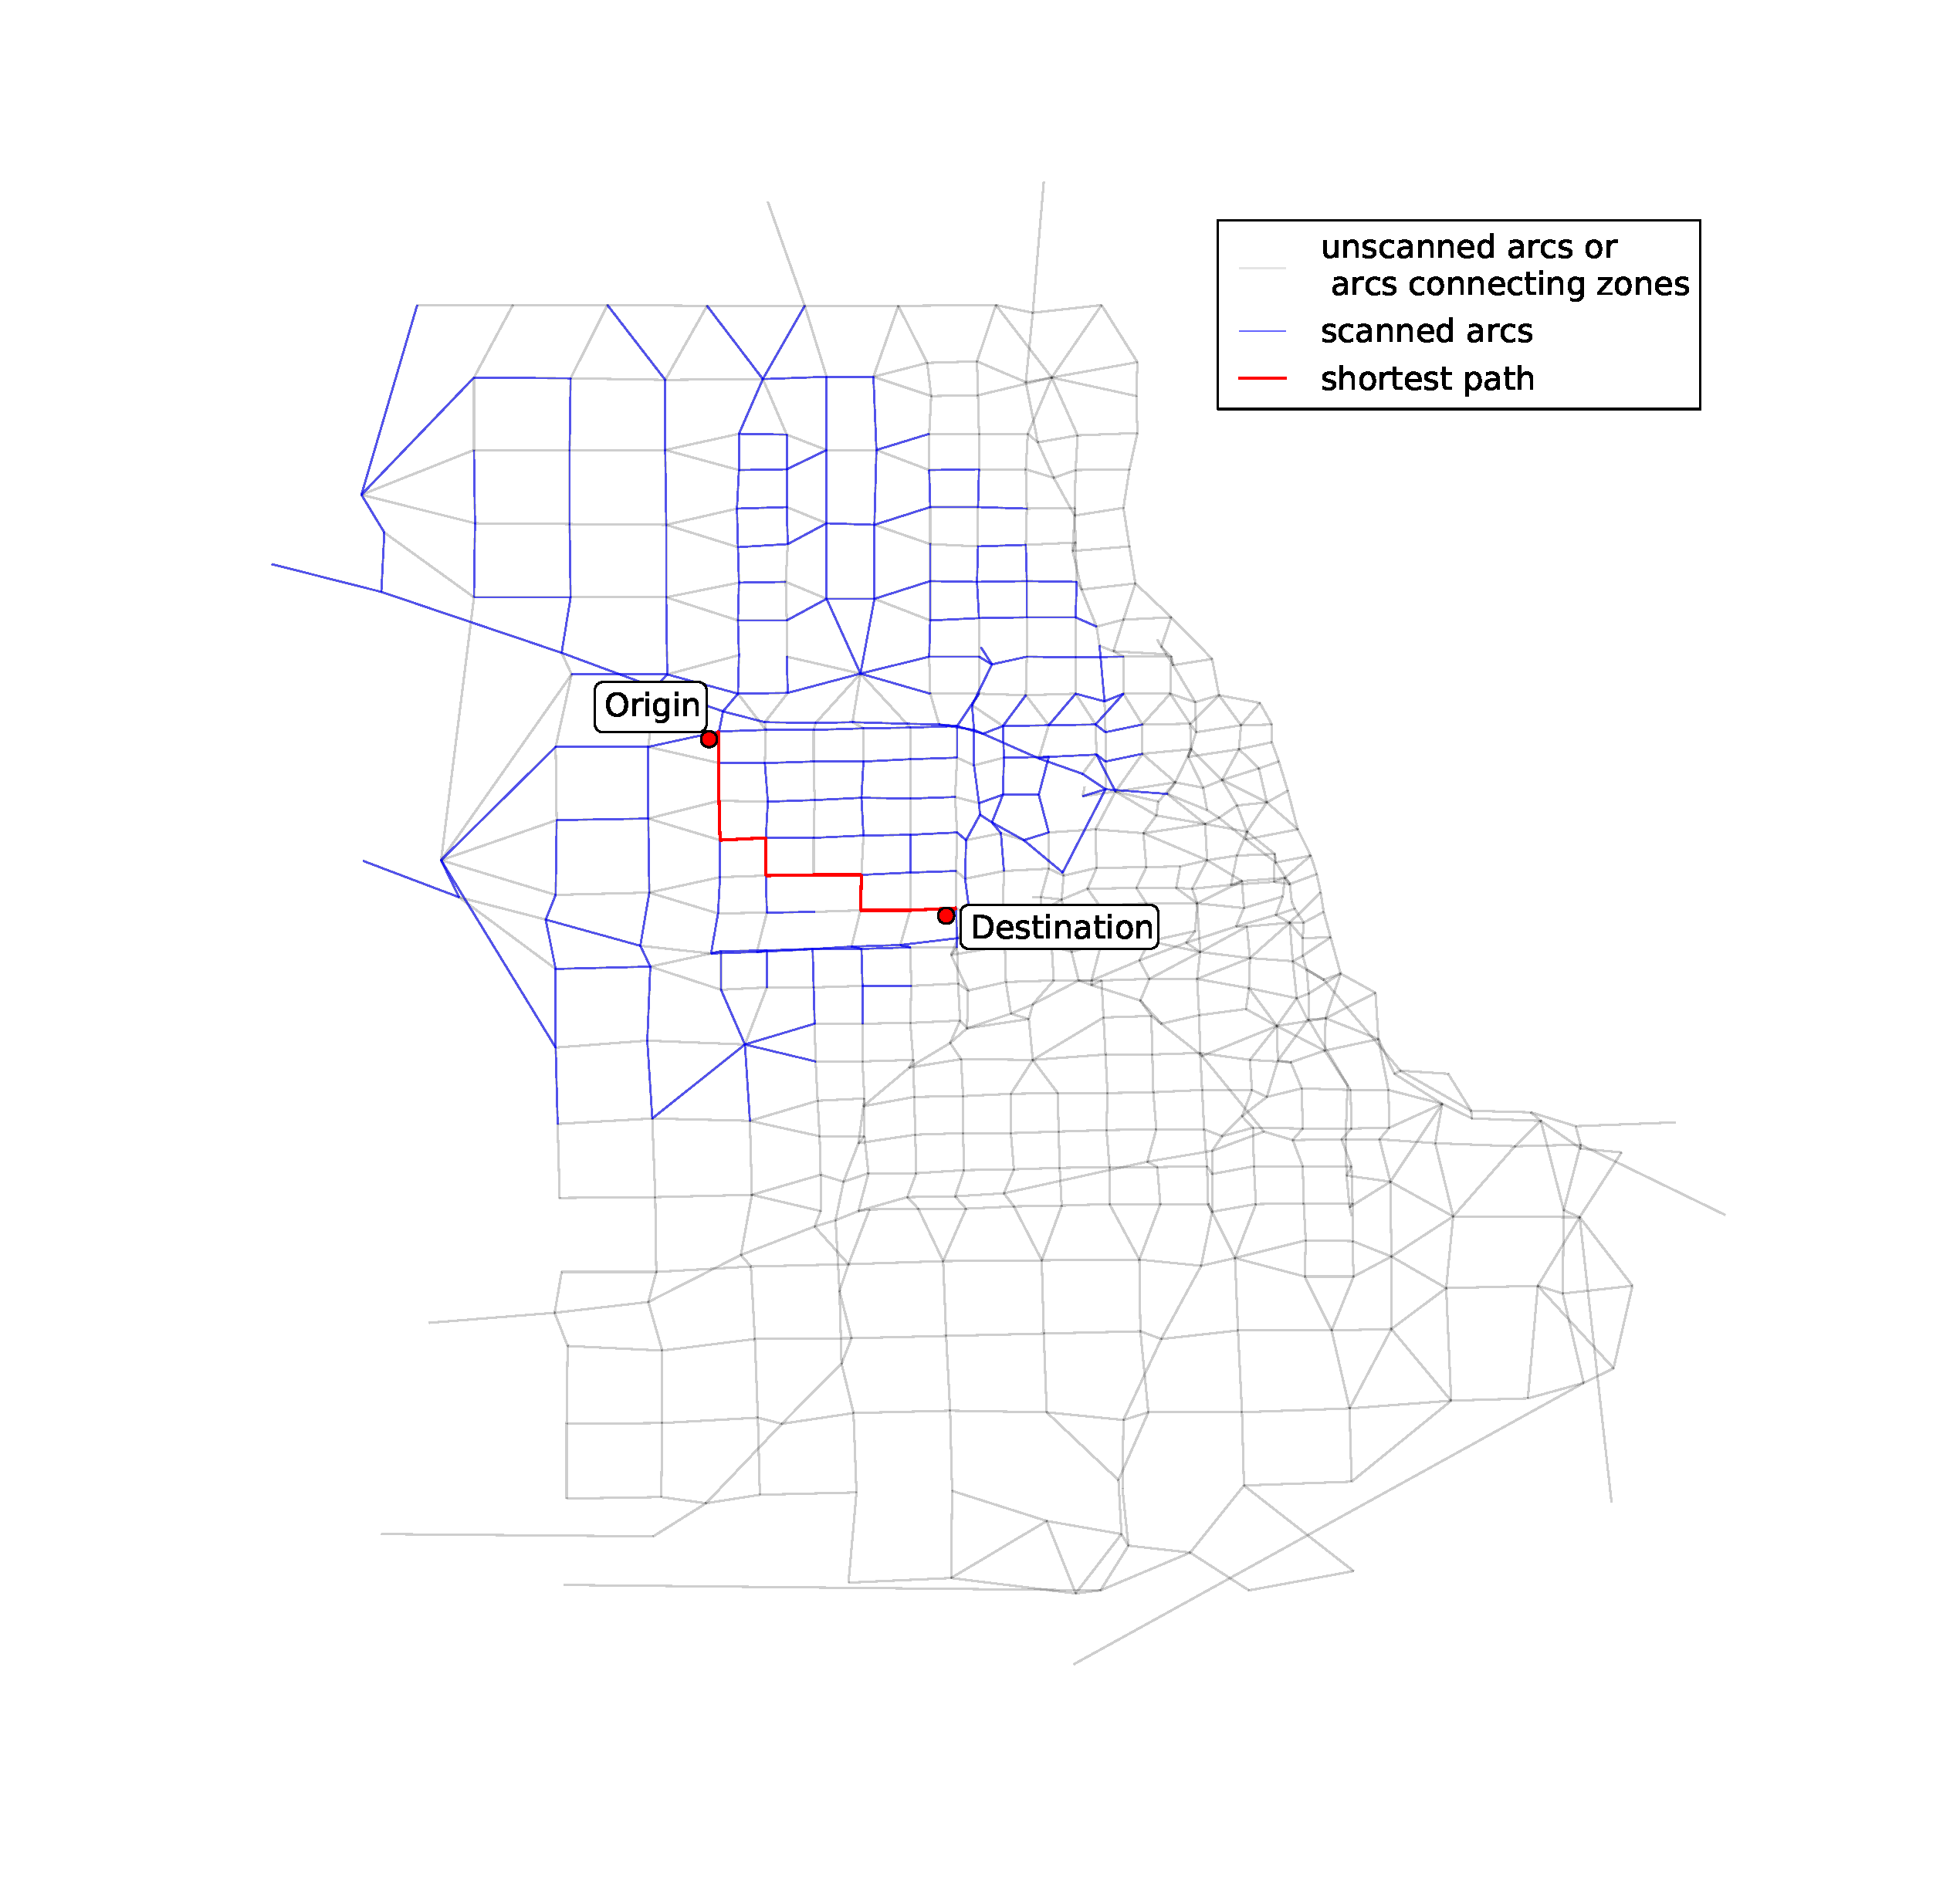
\includegraphics[width=\textwidth,trim=120px 120px 48px 120px,clip]{img/chicago_dijkstra2}
        \caption{Dijkstra}
        \label{fig:chicago_dijkstra2}
    \end{subfigure}%
    \begin{subfigure}{.5\textwidth}
        \centering
        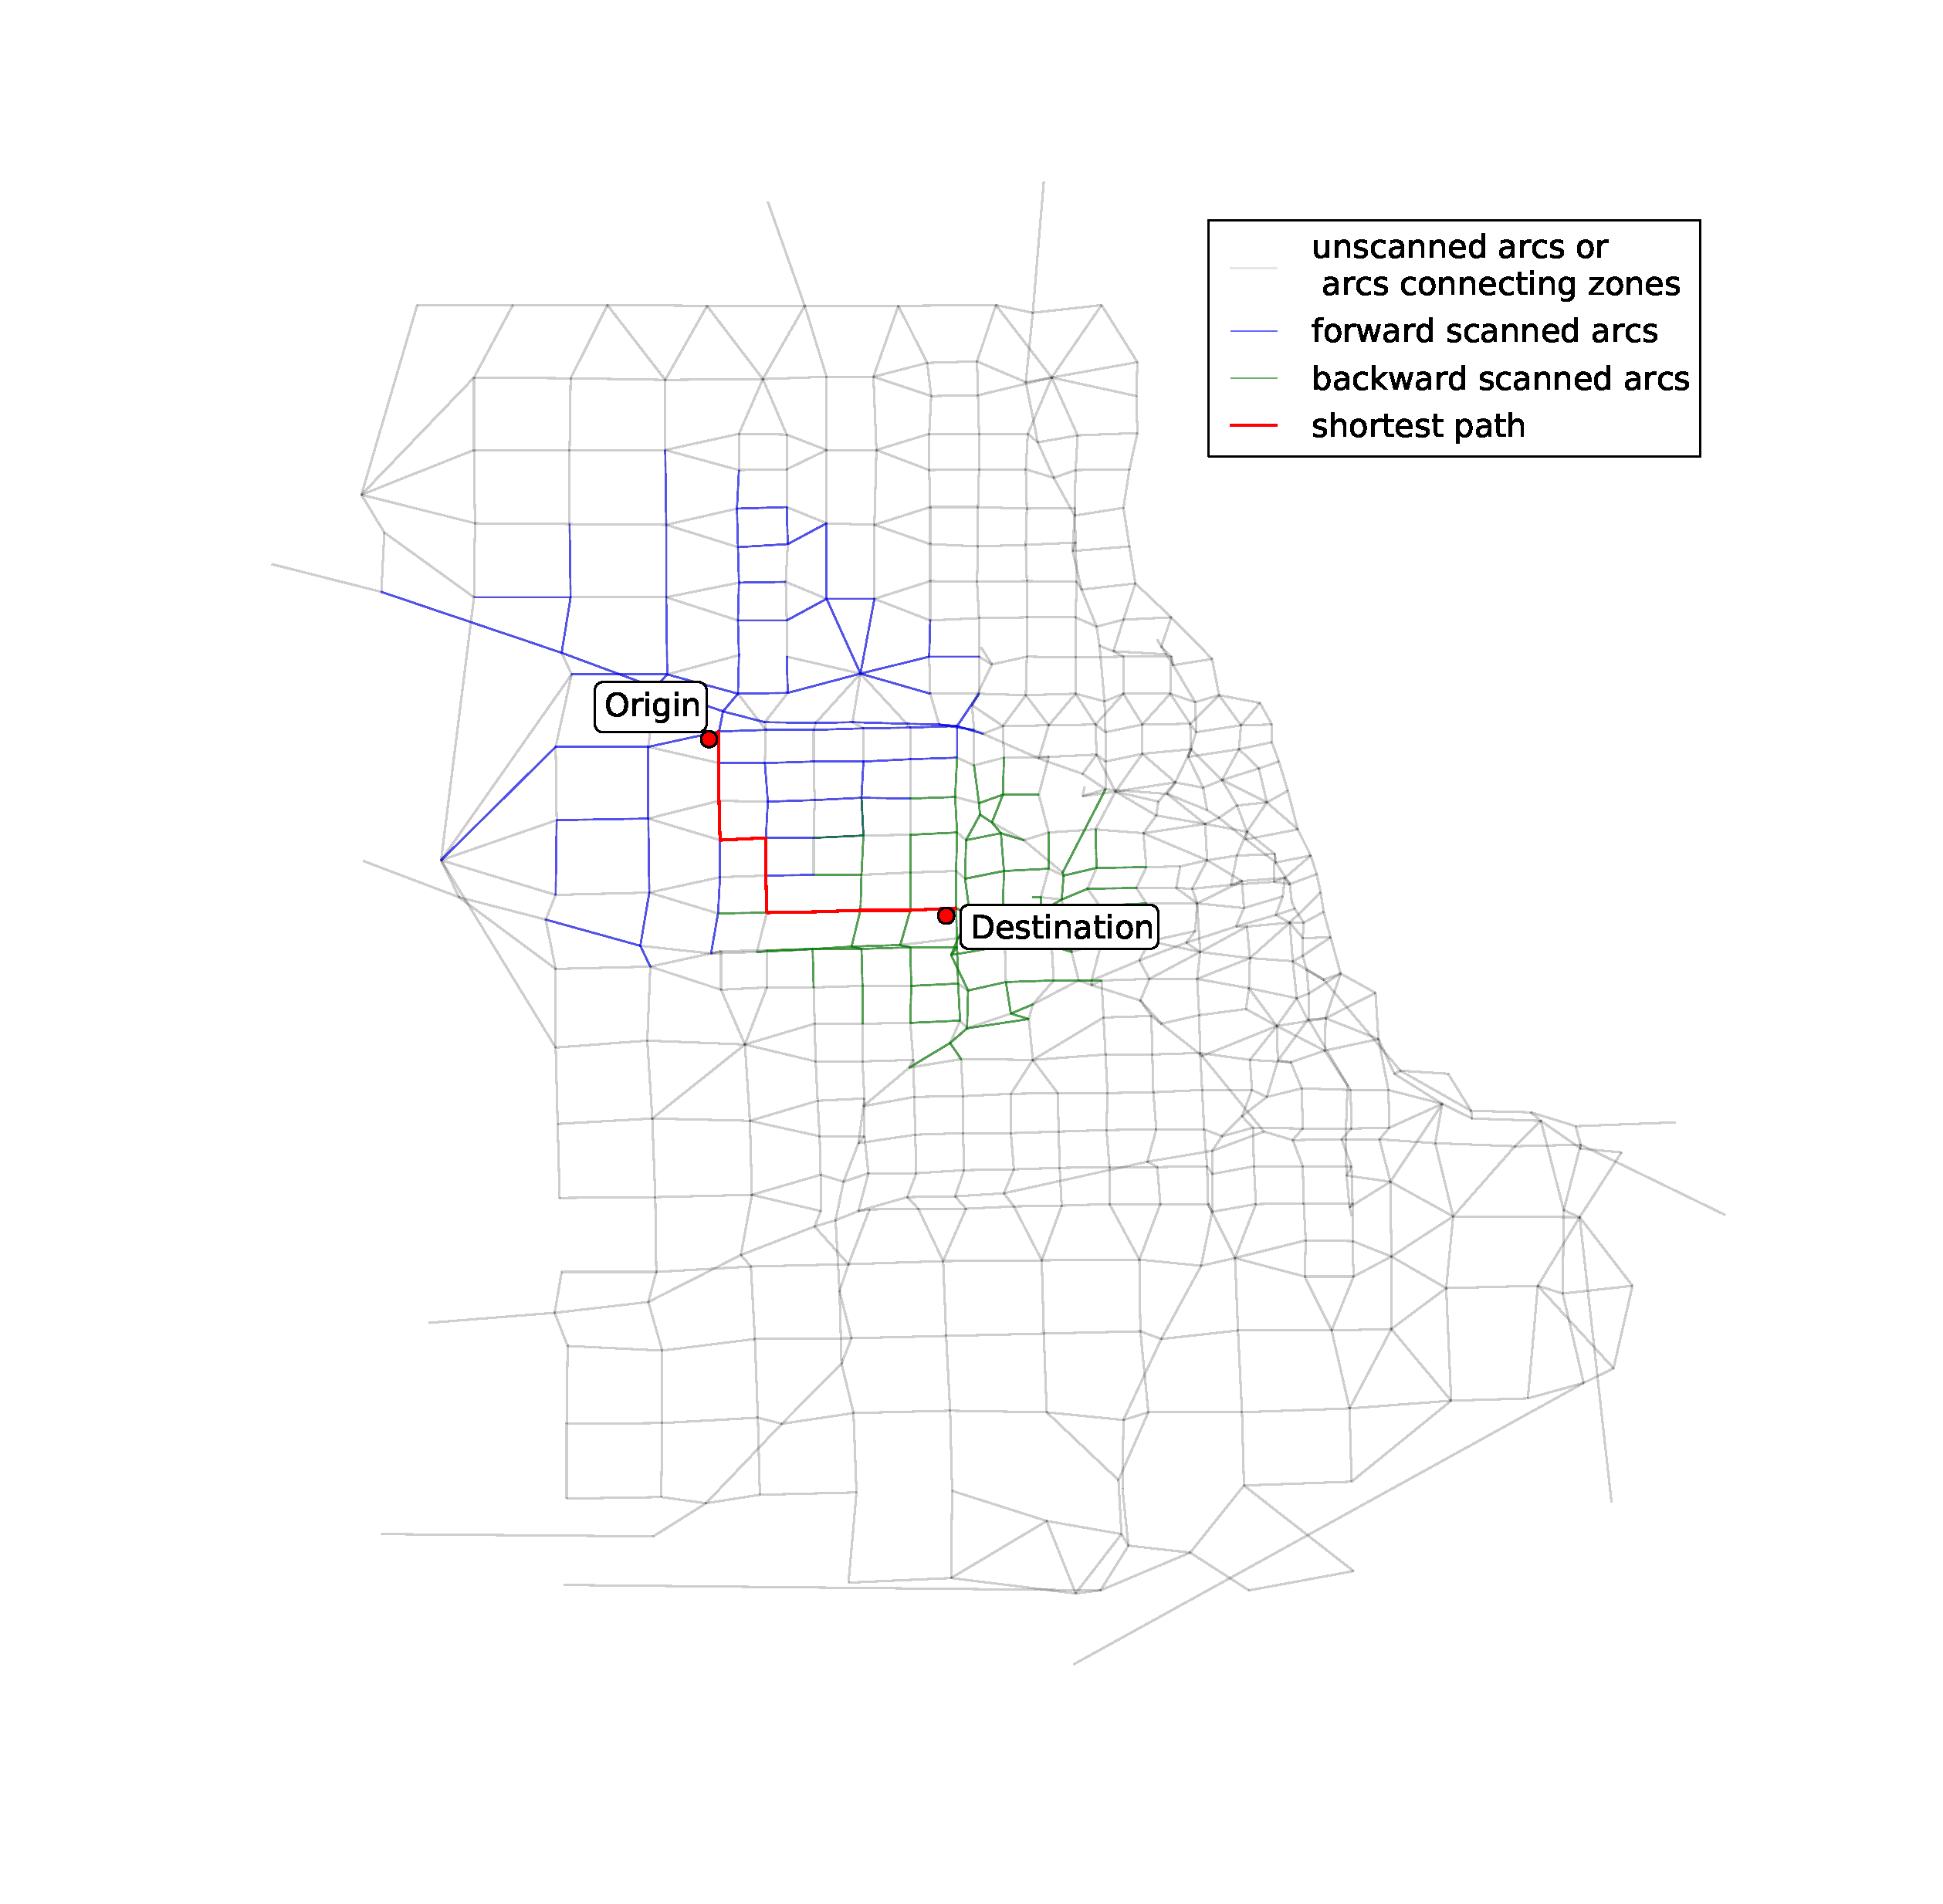
\includegraphics[width=\textwidth,trim=120px 120px 48px 120px,clip]{img/chicago_bidirect2}
        \caption{Bidirectional Dijkstra}
        \label{fig:chicago_bidirect2}
    \end{subfigure}
    \begin{subfigure}{.5\textwidth}
        \centering
        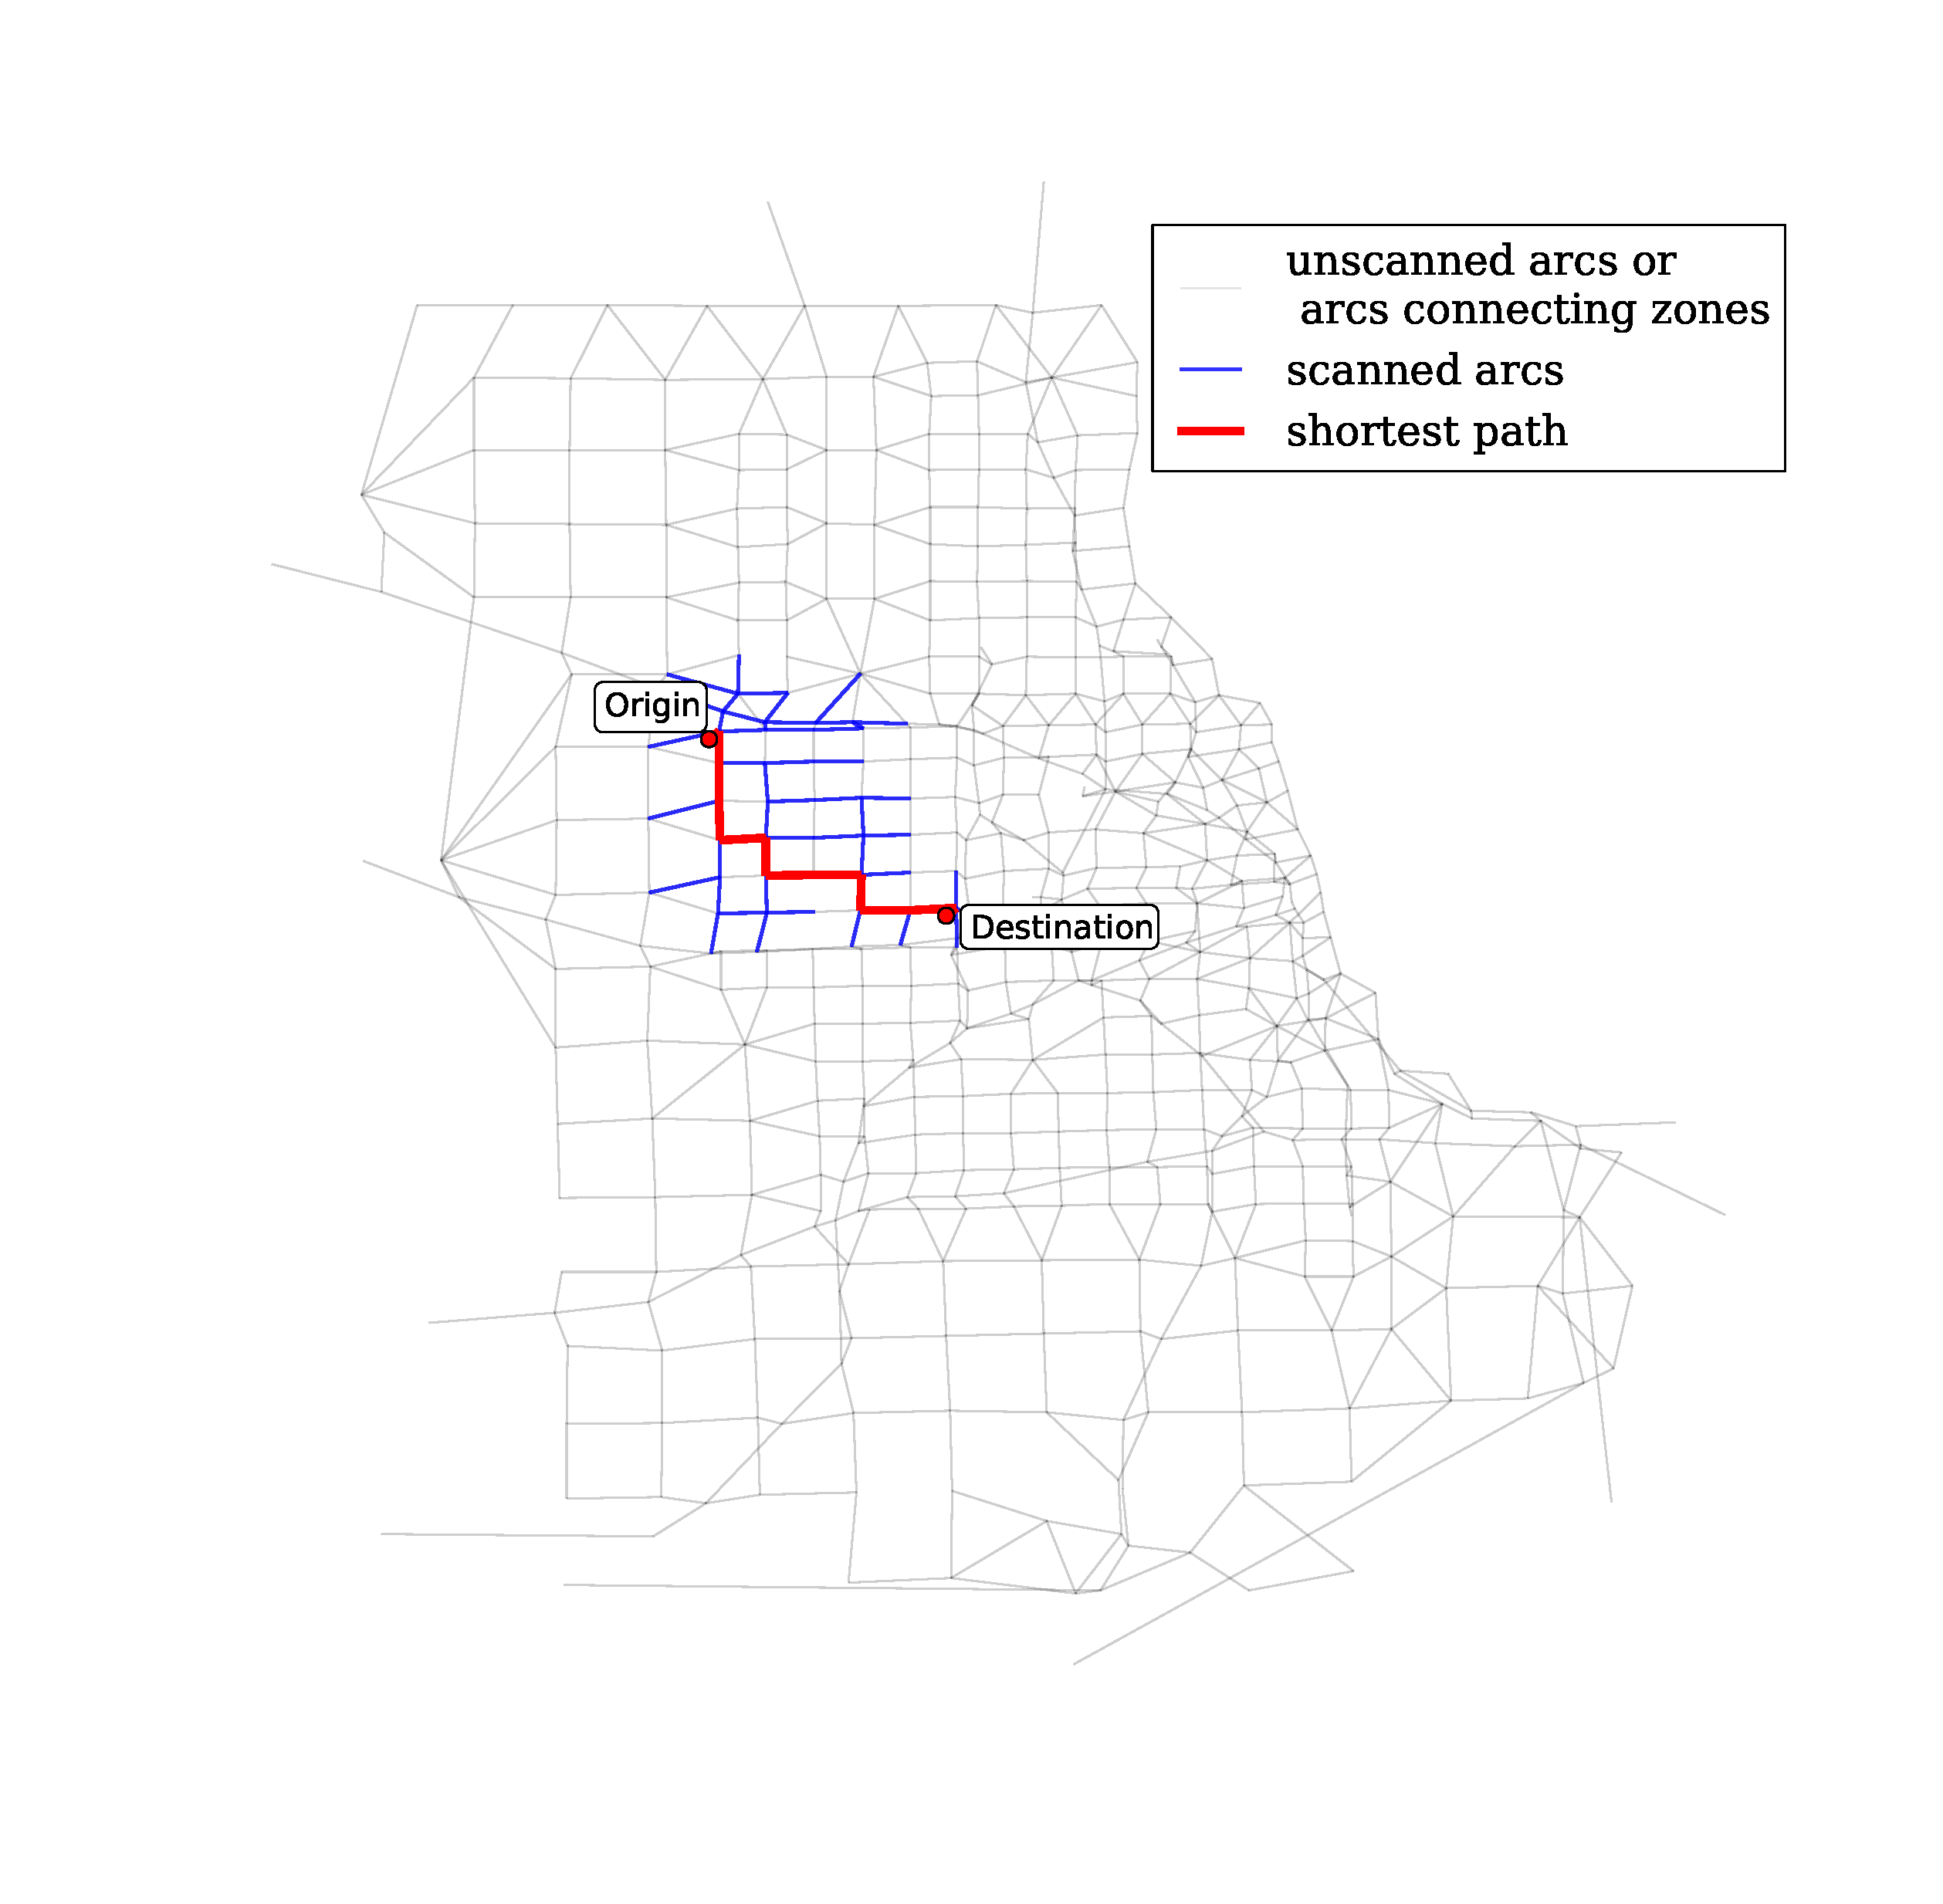
\includegraphics[width=\textwidth,trim=120px 120px 48px 0px,clip]{img/chicago_astar2}
        \caption{A* Search}
        \label{fig:chicago_astar2}
    \end{subfigure}%
    \begin{subfigure}{.5\textwidth}
        \centering
        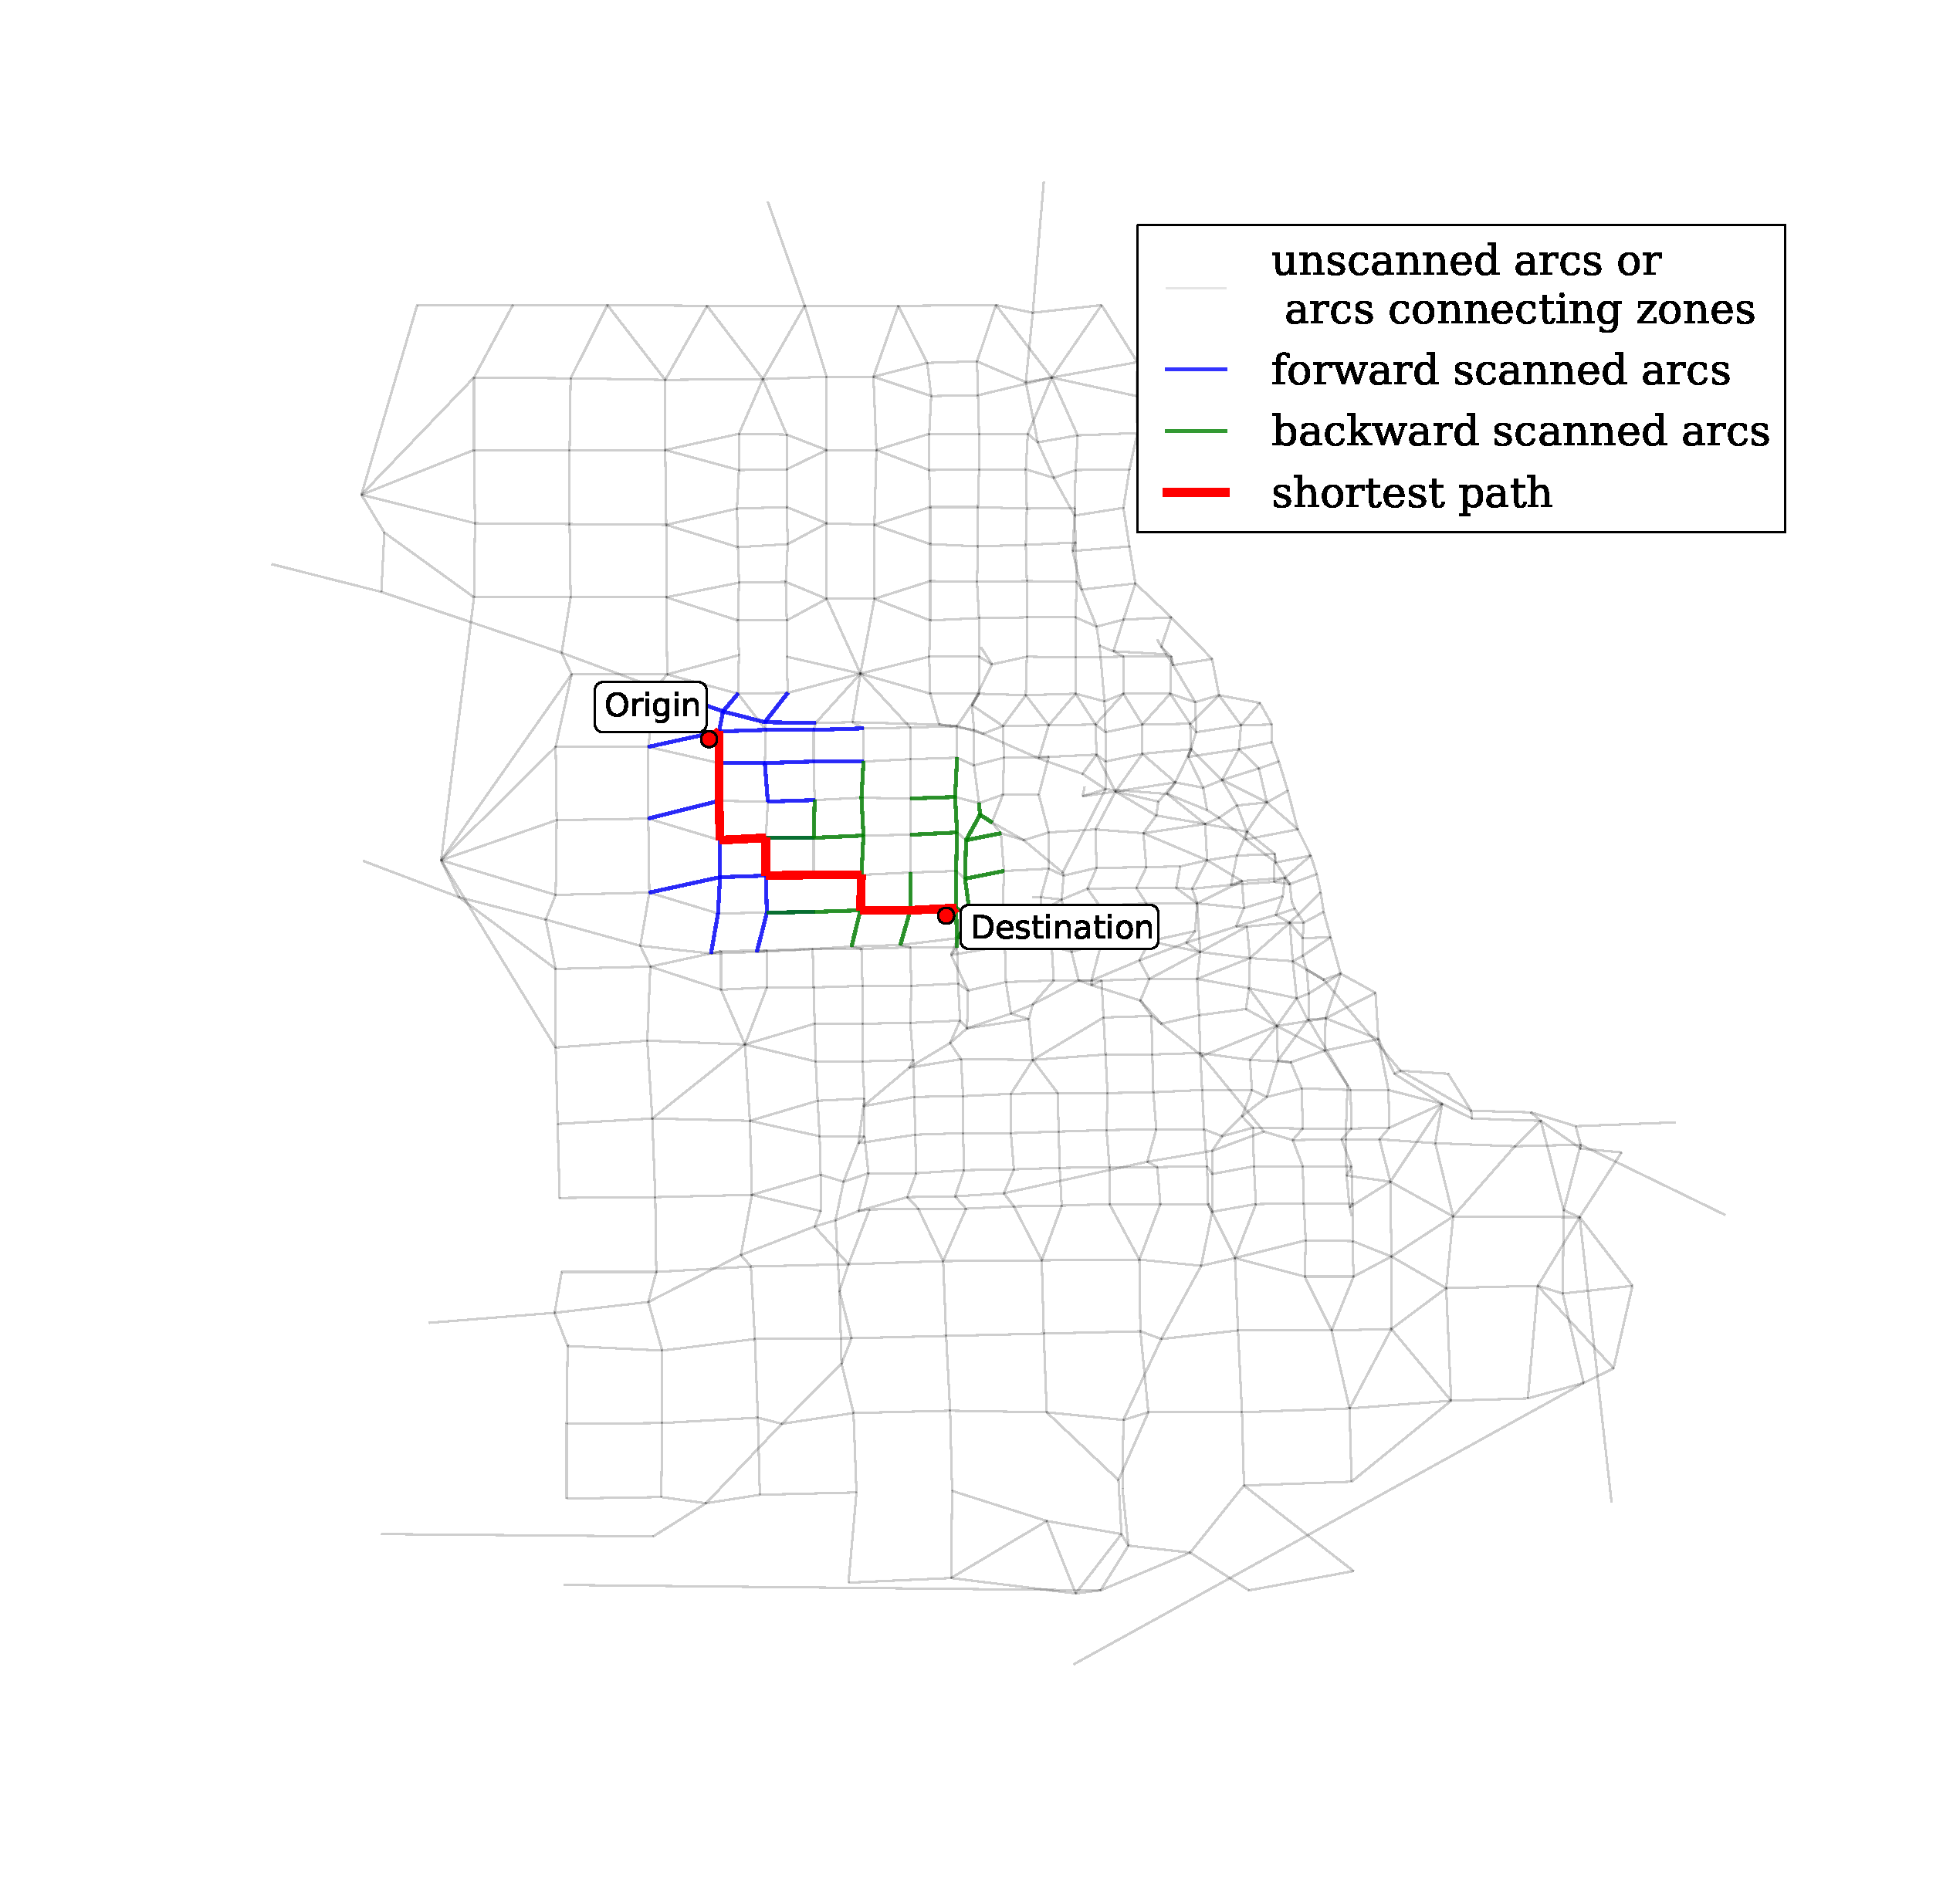
\includegraphics[width=\textwidth,trim=120px 120px 48px 0px,clip]{img/chicago_astar_bidirect2}
        \caption{Bidirectional A* Search}
        \label{fig:chicago_astar_bidirect2}
    \end{subfigure}
    \vspace{1em}
    \caption{Shortest path tree between two close nodes in the ChicagoSketch Network}
    \label{fig:short_sptree}
\end{figure}

\section{A* search with landmarks}
A* search with landmarks algorithm is not implemented for this project.
This is due to two reasons.
The first reason is due to its sophisticated graph dependent implementation,
where we need to either manually or dynamically decide the number of landmarks and their placement locations.
The second reason is due to its high chance of not being able to work,
as the algorithm is aimed at geographic node locations and Euclidean distances,
not our travel times that based on traffic flows.

Preprocessing algorithms are not really practical for the traffic assignment problem and the transportation forecasting model.
This is because normally these algorithms tend to spend much longer time than just running its standard version.
And since the purpose of the traffic assignment is to modify the network and resolve the problem to see its affect on congestion,
so it is not ideal to rerun the preprocessing algorithm every time the network is modified.
